\documentclass[11pt]{article}
\usepackage[margin=1in]{geometry}
\usepackage{booktabs}
\usepackage{graphicx}
\usepackage{hyperref}
\usepackage{amsmath}
\title{PI-MCS: Physics-Informed Mondrian Conformal Selection\\with an Exact Risk Budget for Aircraft Fuel Estimates}
\author{Research protocol and verified development evidence}
\date{22 October 2026}
\begin{document}
\maketitle

\begin{abstract}
Open flight trajectories enable scalable fuel estimation but omit measured mass,
engine state and, often, winds. Selective use of apparently reliable predictions
can also remove difficult aircraft and long intervals. We specify PI-MCS, a
training-fold-only physics residual model with hierarchical aircraft--phase
Mondrian calibration and exact or robust selection under a calibrated risk
budget. The intended contribution is a jointly evaluated aviation decision
system, not a new conformal or robust-optimization theorem. A verified
metadata-only development benchmark covers 131,530 training intervals, 24,289
calibration intervals and 37,456 previously inspected October intervals. It
establishes reproducible baselines but not PI-MCS or external-validation claims.
\end{abstract}

\section{Research gap}
Physics-guided and weather-enhanced aircraft fuel models already exist, as do
weighted, adaptive, group-conditional and risk-controlling conformal methods.
What remains insufficiently tested is whether these uncertainty tools support a
constrained decision about which open-data fuel estimates to release while
preserving aircraft/phase representation under temporal, route and aircraft
shift. PI-MCS addresses that systems-level gap and will be retained only if the
pre-specified grouped experiments support it.

\section{Method}
For segment $i$, the physics prior uses ISA density, wind-corrected true
airspeed, a parabolic drag polar, Breguet cruise fuel and an energy-balance
climb/descent estimate. Take-off mass, TSFC, $C_{D0}$ and Oswald efficiency are
fit by bounded least squares separately by aircraft type using training folds
only. A gradient-boosting/MLP residual ensemble estimates
$\widehat F_i=F_{\mathrm{phys},i}+g(x_i)$ and an out-of-flight-fold model estimates
$\widehat\sigma(x_i)$.

The calibration score is
\[
 s_i=\frac{|F_i-\widehat F_i|}{\max(\widehat\sigma(x_i),\epsilon)}.
\]
Quantiles are estimated within pre-specified aircraft-type $\times$ phase cells,
with hierarchical fallback to aircraft, phase and global calibration. Intervals
are clipped to $[0,\text{tank capacity}]$. Standard split conformal, CQR,
weighted conformal and adaptive conformal are mandatory comparisons.

Selection solves
\[
 \max_{z\in\{0,1\}^N}\sum_i u_i z_i\quad\text{s.t.}\quad
 \sum_i r_i z_i\le B,\qquad \sum_i z_i\ge \lceil mN\rceil.
\]
A Bertsimas--Sim variant protects the risk constraint against up to $\Gamma$
adverse risk deviations. Exact solutions are compared with Lagrangian, greedy,
risk-ranked and conformal-selection baselines. Solver optimality is distinct
from statistical validity.

\section{Development dataset and evidence boundary}
The PRC 2025 benchmark combines ACARS-derived fuel-on-board differences with
OpenSky trajectories and metadata. Its 15,761 flights and 193,275 intervals span
April--October 2025 and 27 aircraft types. Airlines are anonymized and label
unit inference used a broad OpenAP plausibility check. October labels had already
been examined in the inherited project, so all results below are exploratory.

\section{Verified metadata-only baselines}
\begin{table}[ht]
\centering
\caption{Real-data exploratory point-prediction results. Confidence intervals
resample complete route clusters.}
\begin{tabular}{lrrrr}
\toprule
Method & MAE (kg) & Route-cluster 95\% CI & RMSE (kg) & $R^2$ \\
\midrule
Histogram gradient boosting & 79.22 & [67.15, 95.25] & 236.81 & 0.906 \\
Deep ensemble & 79.48 & [67.36, 95.49] & 237.50 & 0.905 \\
MLP & 84.48 & [72.66, 101.08] & 242.19 & 0.901 \\
Aircraft-type median rate & 89.30 & [77.03, 105.24] & 249.36 & 0.895 \\
Quantile regression & 96.18 & [84.04, 112.53] & 246.79 & 0.898 \\
Lasso & 185.22 & [164.80, 209.11] & 404.56 & 0.725 \\
Ridge & 185.23 & [164.81, 209.12] & 404.57 & 0.725 \\
\bottomrule
\end{tabular}

\end{table}

\begin{table}[ht]
\centering
\caption{Ninety-percent interval results calibrated on September 2025.}
\begin{tabular}{lrrr}
\toprule
Method & Coverage & Mean width (kg) & Winkler score \\
\midrule
Histogram gradient boosting & 90.92\% & 293.20 & 858.77 \\
Deep ensemble & 91.01\% & 293.58 & 864.28 \\
MLP & 90.95\% & 331.09 & 865.10 \\
Aircraft-type median rate & 90.93\% & 345.91 & 943.75 \\
Quantile regression & 91.21\% & 395.25 & 909.18 \\
Lasso & 89.97\% & 541.67 & 1742.33 \\
Ridge & 89.97\% & 541.60 & 1742.38 \\
CQR & 89.68\% & 304.85 & 548.03 \\
\bottomrule
\end{tabular}

\end{table}

\begin{figure}[ht]
\centering
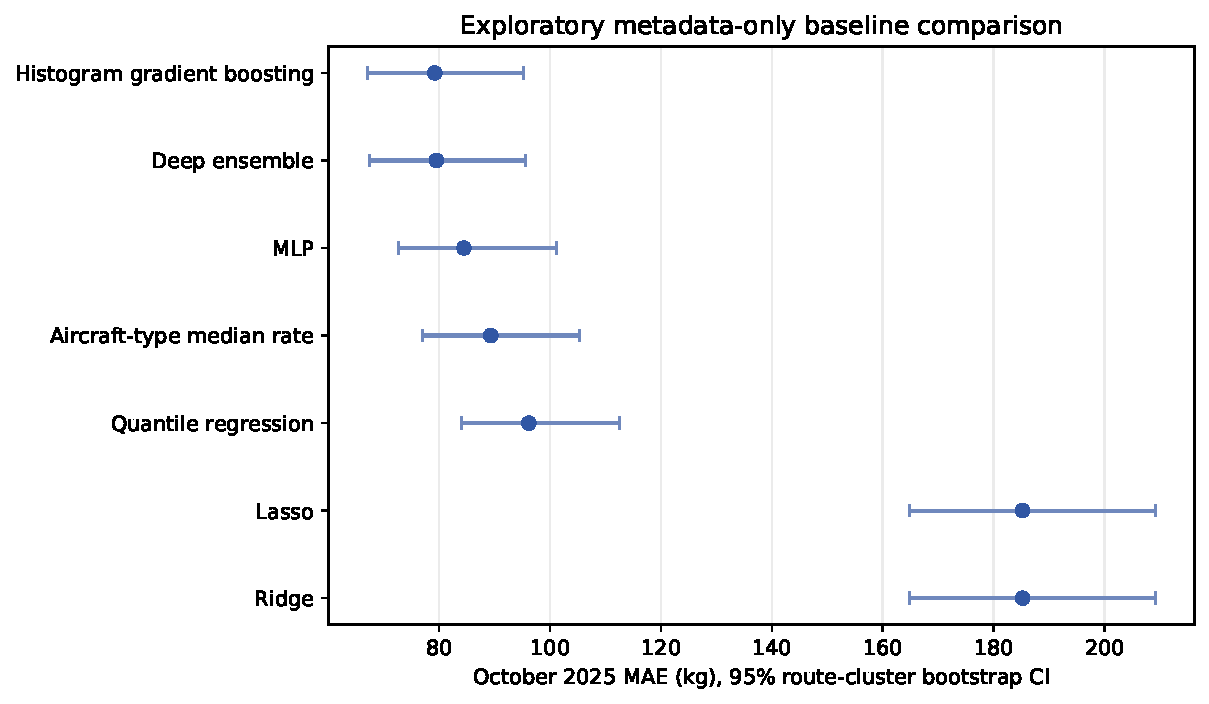
\includegraphics[width=.9\linewidth]{generated/figures/metadata_baselines.pdf}
\caption{Metadata-only October performance. Overlapping intervals must not be
interpreted as evidence of equivalence.}
\end{figure}

Only four test intervals belong to an aircraft type absent from training. This
is inadequate evidence for unseen-aircraft generalization. The full physics,
weather, trajectory, shift, ablation and external-confirmation analyses require
their documented licensed inputs and are not replaced with simulated results.

\section{Validation and statistical analysis}
All observations from one flight remain together. Primary partitions are
forward temporal, route-held-out, aircraft-held-out and aircraft-family-held-out,
with grouped inner cross-validation. We report MAE, RMSE, marginal and
conditional coverage, width, Winkler score, ECE, Brier score, selected-set
coverage, utility, violation rate, solver gap/time and missingness sensitivity.
Confidence intervals resample route or aircraft clusters. Confirmatory tests use
paired bootstrap or Wilcoxon tests, effect sizes and Holm correction.

\section{Limitations and claims}
No universal conditional-coverage, live-operation, airline-level, multi-year or
external-validity claim follows from the current benchmark. Weighted conformal
validity requires correct density ratios; adaptive conformal offers an online
frequency statement; conformal selection requires its exact exchangeability and
dependence assumptions. A dashboard is not evidence. Hypotheses are reported as
pass, fail or inconclusive, including negative results.

\section{Data and code availability}
The development dataset is available under CC BY 4.0 at
\url{https://doi.org/10.5281/zenodo.19184662}. This additive extension records
source hashes, configurations and fixed seeds. OpenSky historical and ERA5 data
must be obtained under their respective access and license terms. No protected
future-confirmation labels are included or opened. The upstream software did not
carry a license in this fork; redistribution requires the upstream author's
permission.

\end{document}

